% withpage: ページ番号をつける (著者確認用)
% english: 英語原稿用フォーマット
\documentclass{ipsjprosym}
%\documentclass[withpage,english]{ipsjprosym}

\usepackage[dvips]{graphicx}
\usepackage{latexsym}

\begin{document}

\title{検索の民主化}
\affiliate{Keio}{慶應義塾大学 環境情報学部}
\author{増井 俊之}{Toshiyuki Masui}{Keio}[masui@pitecan.com]

\long\def\ds{DemocraSearch}

\begin{abstract}
  検索エンジンの検索結果はユーザがコントロールできないし、
  非公開の情報やローカルマシンの情報を検索することはできない。
  必要な情報がWebで公開されている場合でも名前に特徴が無ければ検索が難しいこともある。
  %
  与えたキーワードに対する検索の挙動をカスタマイズできるように検索エンジンを拡張して「民主化」することにより、
  あらゆる種類の情報に同じインタフェースでアクセスできる\textbf{\ds}システムを提案する。
  {\ds}を利用すると、「プロシン」でWeb検索したり、「パスワード」で自分のパスワードを表示したり、
  「天気」で現在地の天気予報を表示したり、
  「住所」で自分に関係する住所のリストを表示したり、
  あらゆる情報に同じインタフェースでアクセスできるようになる。
  %
  本論文では、{\ds}の実装と利用例について述べる。
\end{abstract}

\begin{jkeyword}
  検索の民主化, {\ds}, 検索, ブックマーク, GoQuick, Oumugaeshi
\end{jkeyword}

\maketitle

% Body %%%%%%%%%%%%%%%%%%%%%%%%%%%%%%%%%
\section{はじめに}

誰もが日常的にWebの検索エンジンを利用しているが、
検索手段や検索結果をユーザがコントロールすることができないという問題がある。
一般的なWeb検索エンジンを使った場合、
Web上のデータが自分にとって重要であり検索キーワードが自明な場合でも、
そのキーワードでの検索が成功するとは限らない。
たとえばお気に入りの店の情報がWebで公開されている場合でも、
特徴的な名前でない場合は検索が難しい。
自分や家族に関連する情報がSNSなどで公開されていた場合でも、
名前で検索したときその情報が得られることは稀である。
有名なものや流行しているもの、
検索エンジンが検索させたいものばかりが優遇されていることになる。

当然ではあるが、非公開の情報を検索することはできないし、
自分だけの特殊な略称を使って検索することはできない。
秘密情報をクラウド上に置いている場合でも、
検索エンジン以外の方法でアクセスする必要がある。
パスワード関連の情報をWeb上に公開している場合でも、
「パスワード」というキーワードでその情報にアクセスすることはできない。

% 最近購入した「HHKB」のマニュアルを検索しようとしても、...
% 「HHKBのマニュアル」を捜すのは難しい
%  https://happyhackingkb.com/manual/studio/ug-us/jp/ug/topic/index.html なげーよ

検索しにくい情報や秘密の情報を管理するためには、
個人的なファイルやデータベースを使ったり、
特殊な検索システムを使うのが一般的だと思われる。
性質が異なるデータを捜すときは検索方法が異なるのは
当然だと考えられているかもしれないが、
場合に応じて検索方法を変えるのは面倒である。
情報の種類にかかわらず同じ方法で検索できる方が便利だし、
欲しい情報に最短でアクセスしたい。
検索対象のカテゴリを考えてからキーワード検索をするのは無駄である。

必要な情報について書かれたWebページがみつかった場合でも、
本当に必要な情報がすぐにみつかるとは限らない。
店に電話をかけたいとき、
Web上の店のページの検索に成功したとしても、
電話番号を調べるのは苦労することがある。
住所なども同様である。

与えたキーワードに対する検索の挙動を自由にカスタマイズできるように
検索エンジンを拡張することにより、
自分が必要とするあらゆる情報に同じインタフェースで効率良くアクセスすることができる。
このようなことを可能にする\textbf{\ds}システムを提案する。

%  店の電話番号
%  住所を知る
%  「天気」で検索したとき、現在地の天気予報が表示されてほしいが、
%  「地震」で検索したとき、現在の現在地付近の地震情報が表示されてほしいだろう
%  「パスワード」で検索したとき、
%  「プロシン」で検索したとき、2024年のプロシンの投稿方法を知りたい 参加方法を知りたい
%  好きな音楽をキーワードでさがしたり
%  答をすぐに得たり

\section{\ds}

{\ds}は以下の順番で検索を行なう。

% \item 答を直接取得 (これは違うか)

\begin{enumerate}
\item 自分独自のキーワードで検索実行
\item ショートカットの利用
\item 通常のWeb検索
\end{enumerate}

\vspace{2mm}
\noindent
DemocraSearchを利用すると、
自分が必要とする様々なタイプの情報に対して
同じインタフェースでアクセスできるようになる。

\subsection{自分独自のキーワードで検索}
\label{mykw}

{\ds}では、
展開ヘルプ\cite{expandhelp}の手法で検索文字列を指定できる。
図\ref{register}では、
プロシンのページに対して
\verb+(prosym|プロシン|プログラミングシンポジウム)+
のような正規表現で検索キーワードを指定している。

% プロシンのトップページを「prosym」「プロシン」などのキーワードで検索したい場合、
% {\ds}の登録機能で以下のように登録を行なう。

\begin{figure}[h]
  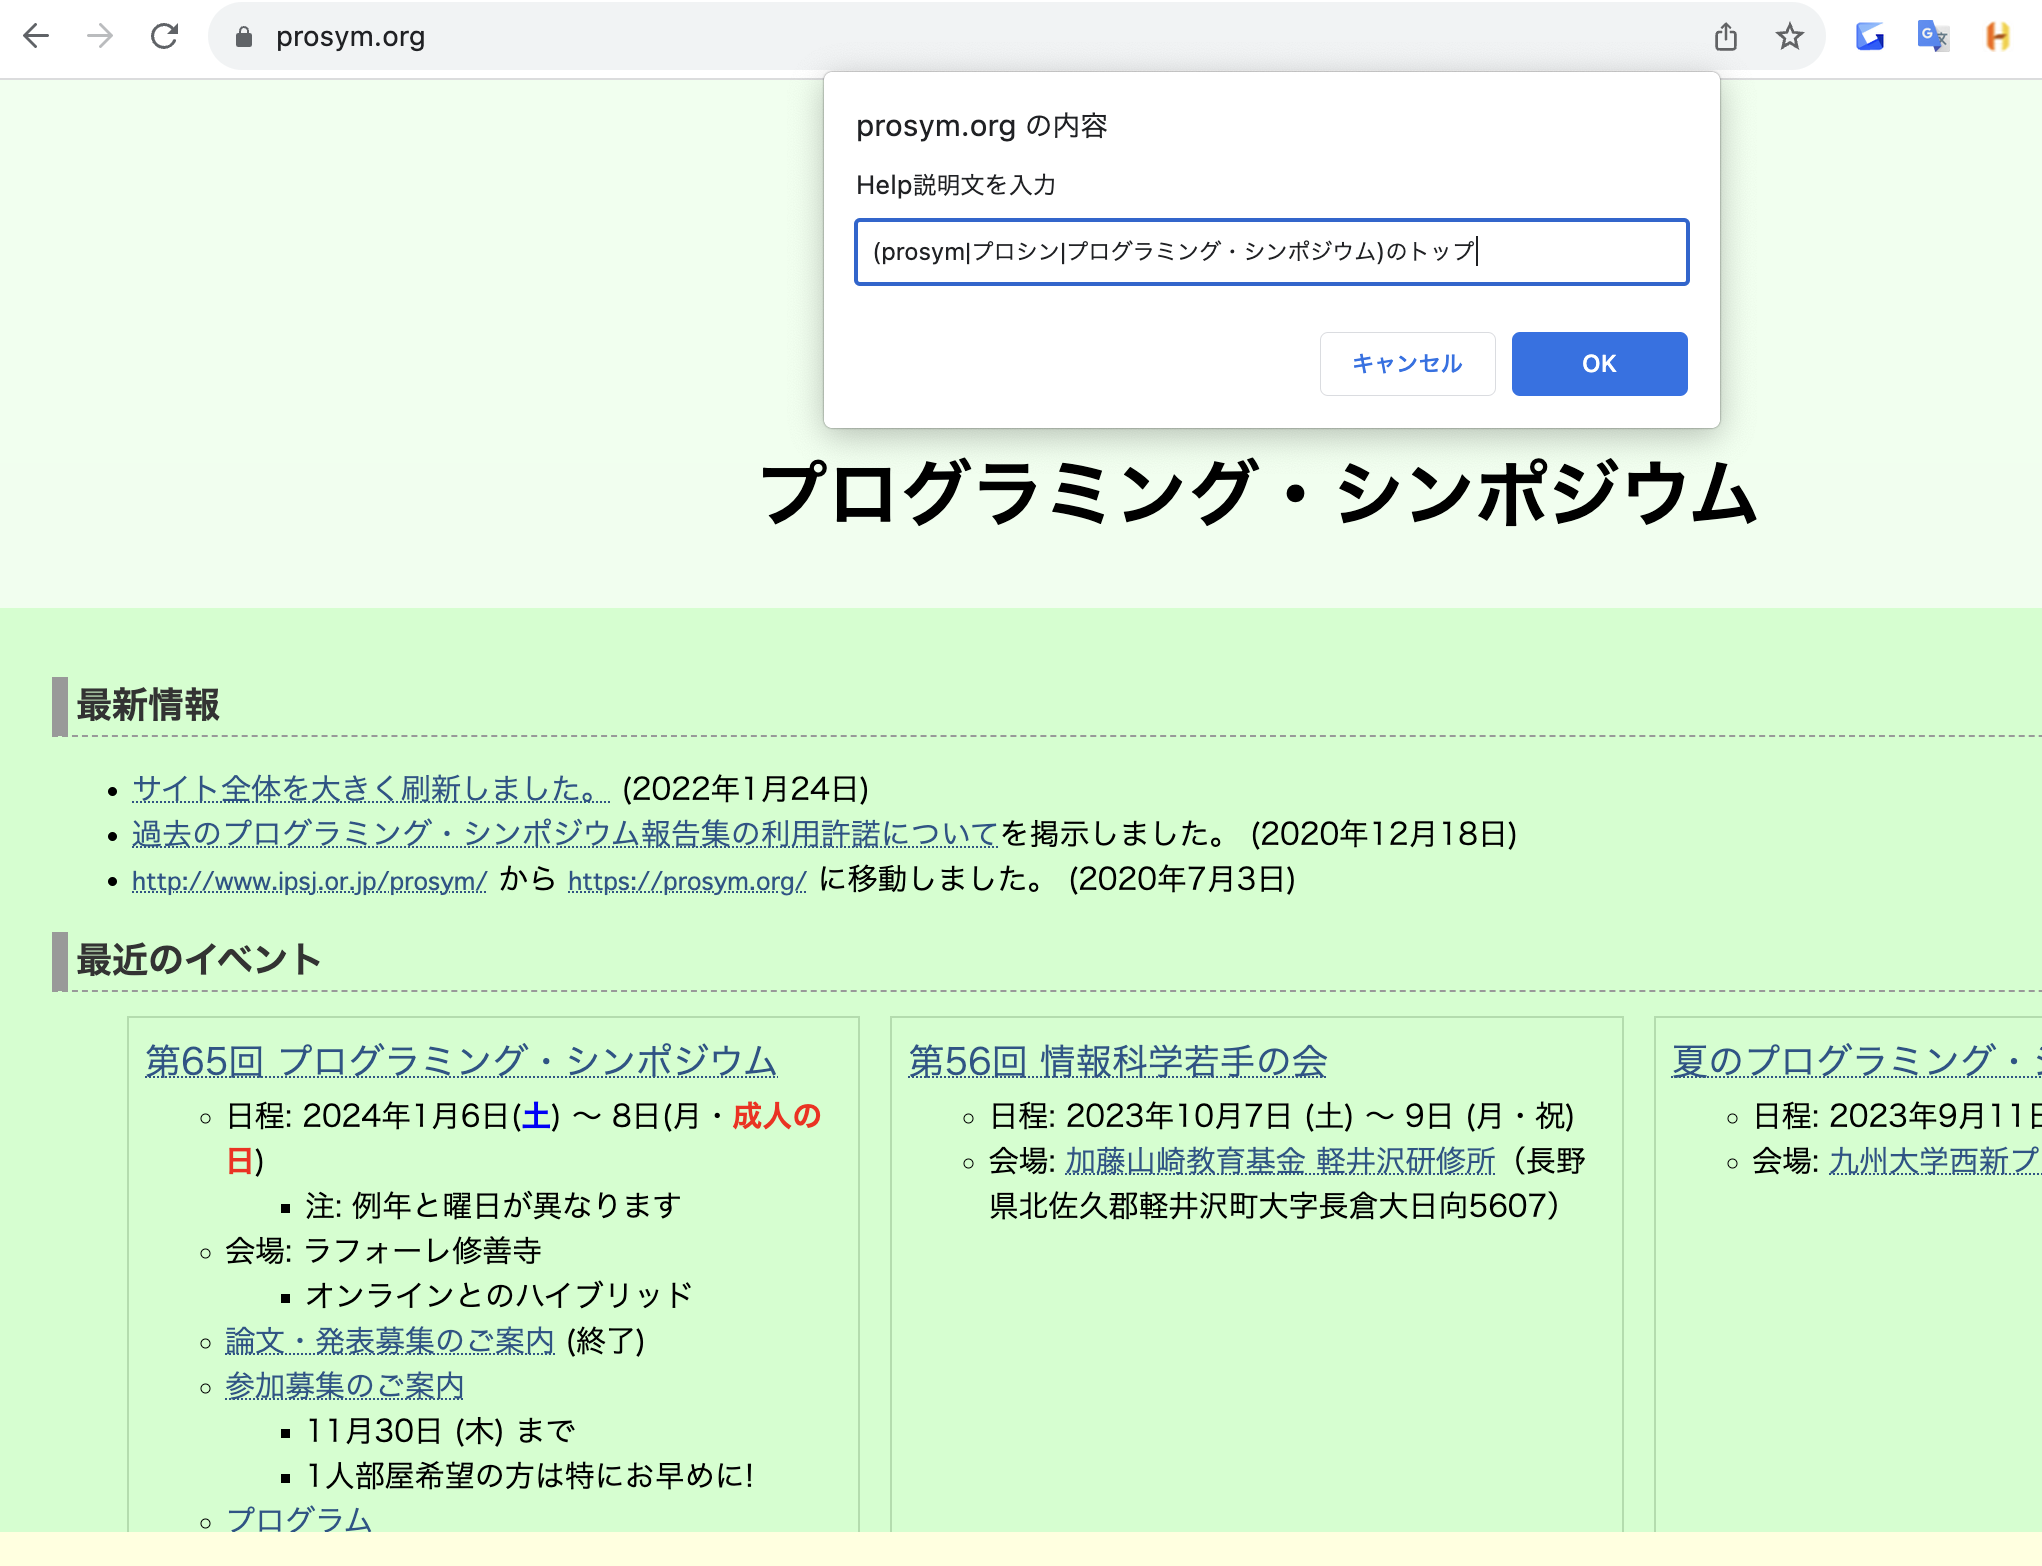
\includegraphics[width=10cm,bb=0 0 2042 1566]{figures/b68d8c865c12932d5cbbea92c2d8605d.png}
  \caption{検索文字列を正規表現で登録.}
  \label{register}
\end{figure}

この状態で「プロ」で検索すると、
図\ref{result}のように検索結果がメニューで表示される。

\begin{figure}[h]
  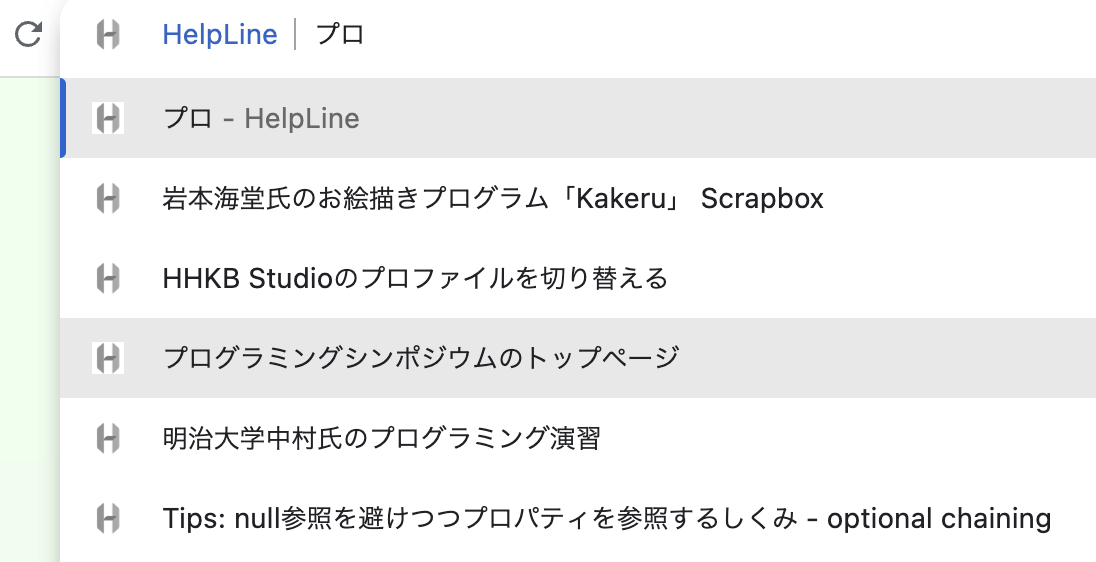
\includegraphics[width=10cm,bb=0 0 1096 562]{figures/502c482135a43d72b8c1ac7d741a68c9.png}
  \caption{「プロ」での検索結果.}
  \label{result}
\end{figure}

会場の地図を「ラフォーレ修善寺の地図」のような名前で登録しておけば、
「ラフォーレ」「地図」などのキーワードからすぐに地図ページにアクセスできる。

% Web上検索を行なう前に自分独自の検索を行ない、マッチするものが無い場合に検索エンジンを利用する
% このためには、検索エンジンのフロントエンド的なものを使えば良い。
%  たとえば「プロシンのページにアクセスしたいとき、
%    まず「プロシン」というキーワードで独自データベースの検索を行ない、結果が無い場合に一般の検索エンジンを利用する。この方法により、自分独自の検索も一般的な検索も同様の作業で検索できることになる。
%  自分独自の検索を行なう場合、検索キーワード
%   たとえば知人の情報を独自キーワードで検索したい場合、苗字やニックネームや関連キーワードで検索できるようにしたいだろう。
%   (秋葉原|末広町)のナントカ電子
%   鎌倉の小町通りの焼き鳥屋「鉄砲串」
%   といった検索文字列を登録しておけばよい。
%  様々なキーワードで検索できるようにするため、なるべく幅広いキーワードで登録をしておくことが望ましい。
%   このために「展開ヘルプ」の手法を利用している。
%   展開ヘルプでは、検索に利用されるフレーズを正規表現で記述する。
%   Helpfeelというものを提案し、広く利用されている 
%  Tipsの例
%   Exifを含まないJPEGファイルに撮影時刻情報を追加する方法
%   ScrapboxページにGyazoのOCRデータを追加する
%   ブラウザやコマンドラインからKindle本を開く
%   Scrapboxに貼ったプログラムをコマンドラインから動かす
%   odコマンドで1バイトずつ、16進数と文字を表示するオプションです
%   gitで2日前のファイルにアクセスする
%   BGMを(流す|再生する)
%   ハウスを再生する

登録したい情報が沢山ある場合は
Scrapbox\footnote{
  \textsf{https://scrapbox.io/product}
}のプロジェクトから一括登録することができる。
慶應SFC\footnote{
  \textsf{https://www.sfc.keio.ac.jp/}
}の学生生活のノウハウを
SFCHelp\footnote{
  \textsf{https://scrapbox.io/SFCHelp/}
}というScrapboxサイトでまとめているが、
この中のページで図\ref{GPA}のような「Helpfeel\footnote{
  \textsf{https://helpfeel.com/}
}記述」をしておくと、その正規表現を検索キーワードとして利用できる。

\begin{figure}[h]
  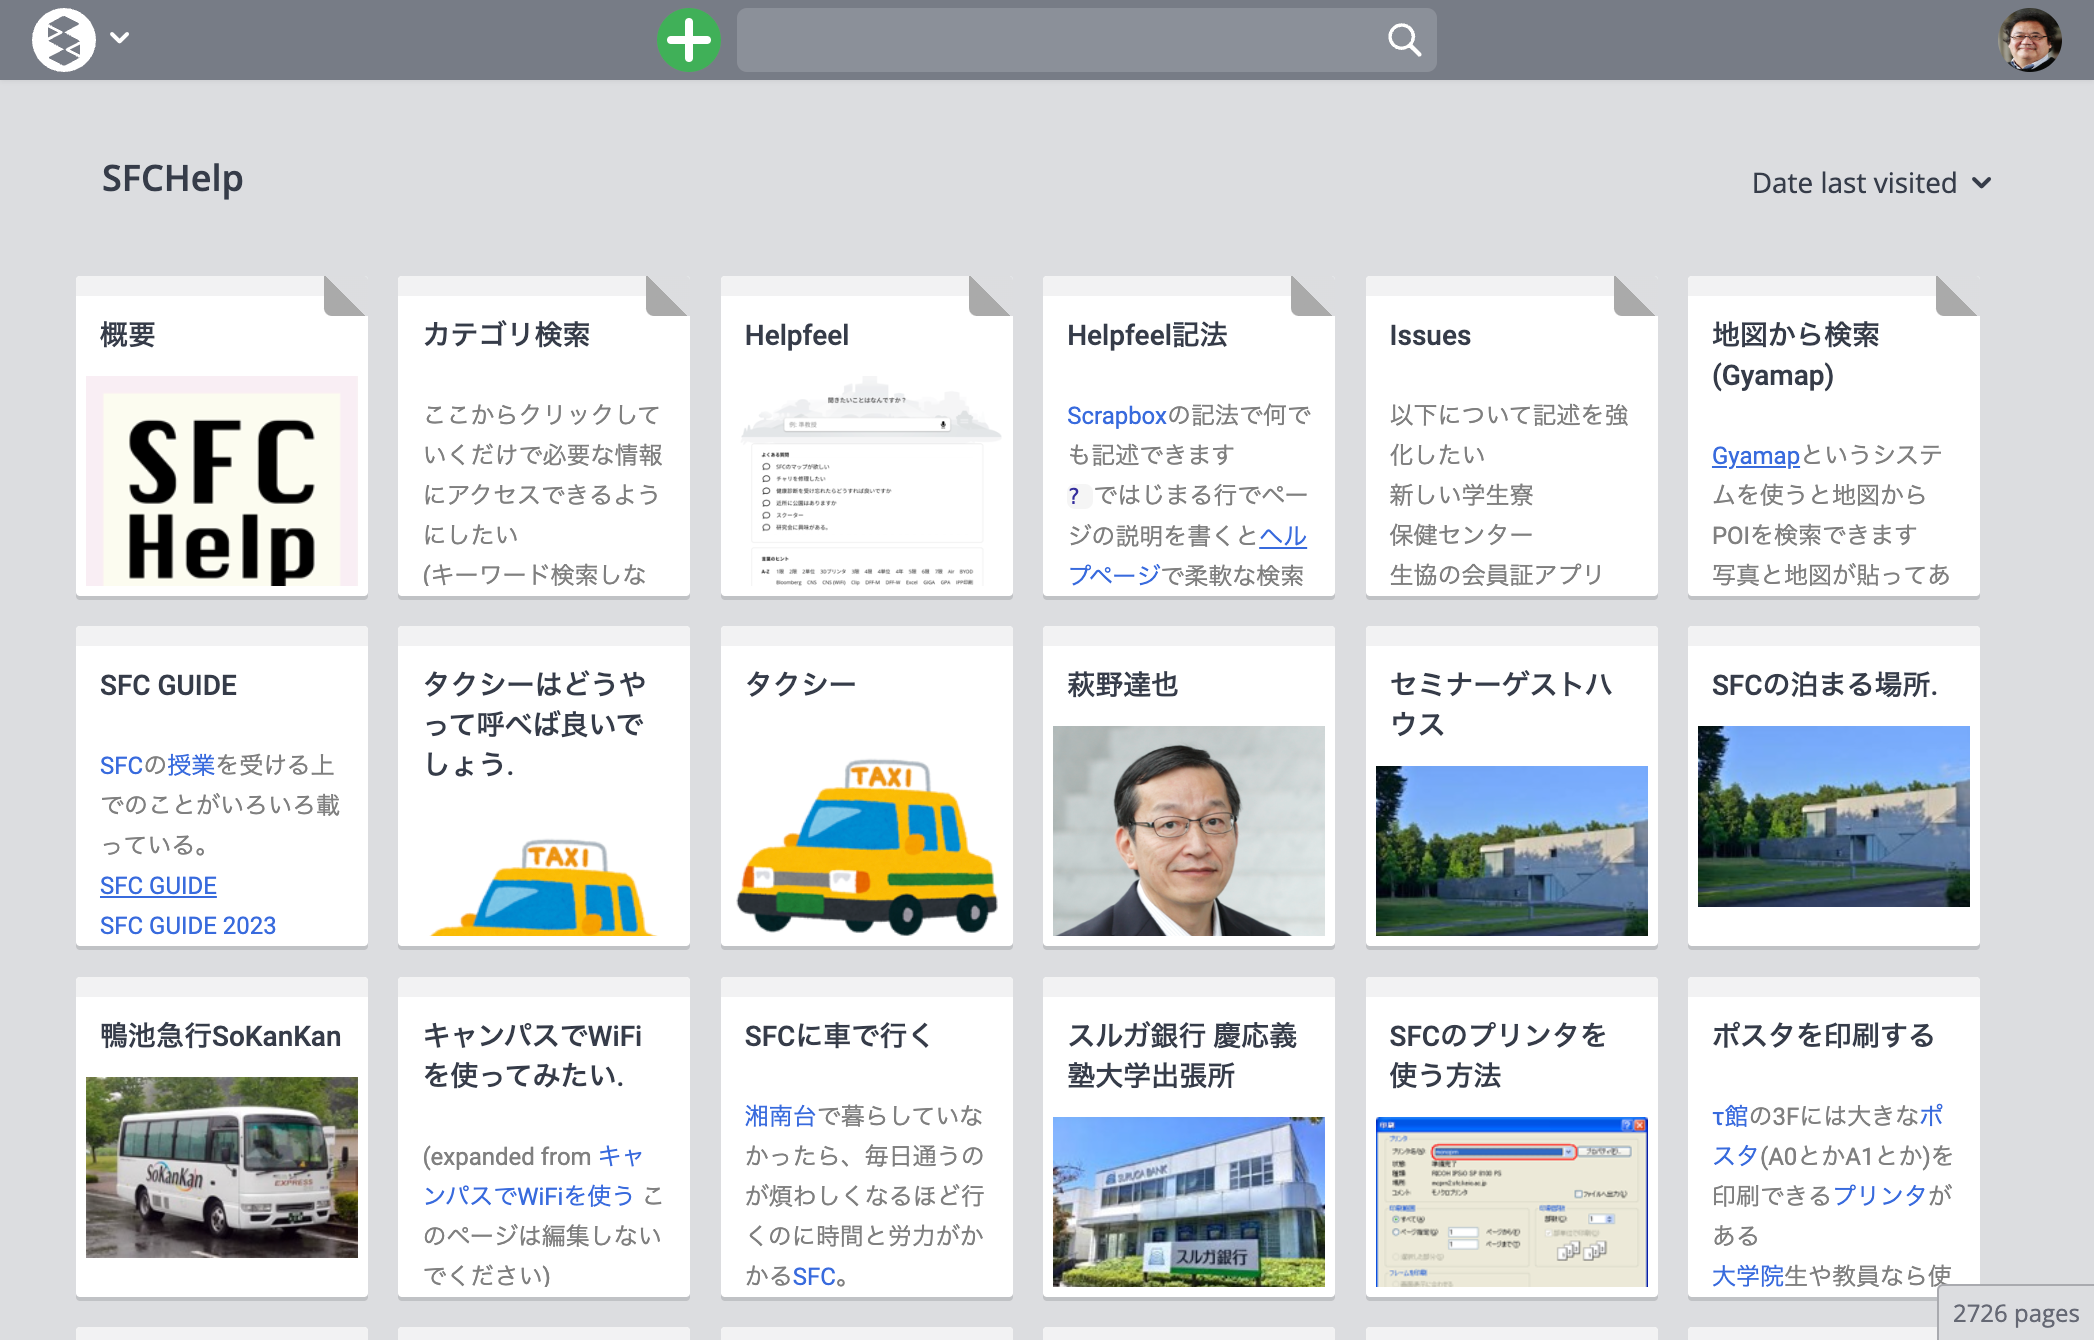
\includegraphics[width=10cm,bb=0 0 2094 1340]{figures/d3953ee26dadc46b4761014664a1c7a3.png}
  \caption{SFCに関する情報共有サイト.}
  \label{sfchelp}
\end{figure}

\begin{figure}[h]
  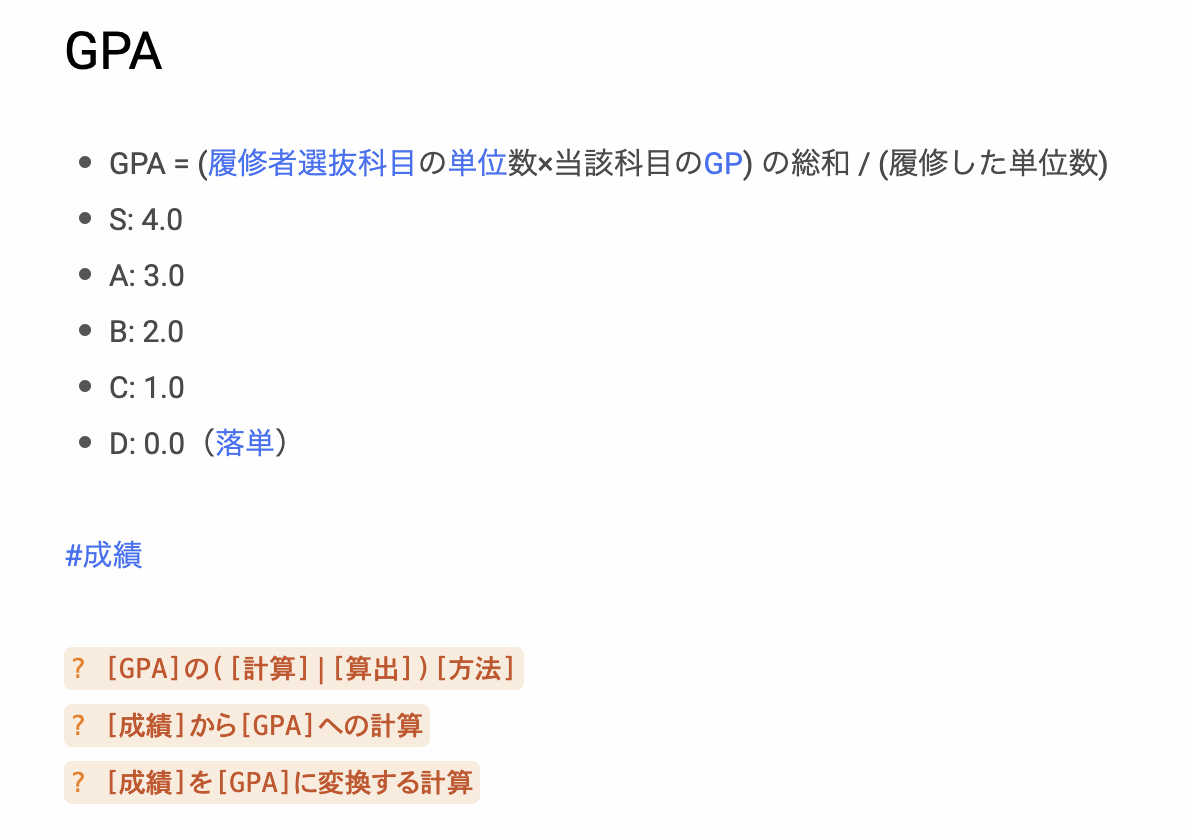
\includegraphics[width=10cm,bb=0 0 1186 836]{figures/34e05297922fbd2133bf4011f97457b8.png}
  \caption{SFCHelpに記載されたGPA情報.}
  \label{GPA}
\end{figure}

\subsection{ブックマークとショートカット}
   
よく使うWebページはブラウザにブックマークすることができるが、
ブックマークの数が多くなるとメニューが巨大化して使いにくくなる。
ここでショートカットキーを利用すると便利である。

GoQuickというサービス\footnote{
  \textsf{http://GoQuick.com/}
}では、様々なWebサイトに対して短い名前を登録し、
その名前を利用してページに直接アクセスすることができる。
たとえば訪問先を示す地図ページを「map」という名前で登録しておけば、
ブラウザのURL入力欄\footnote{
 Chromeブラウザでは「Omnibox」と呼ばれる。
}で「map」と入力することによりで地図にアクセスできる。

\begin{figure}[h]
  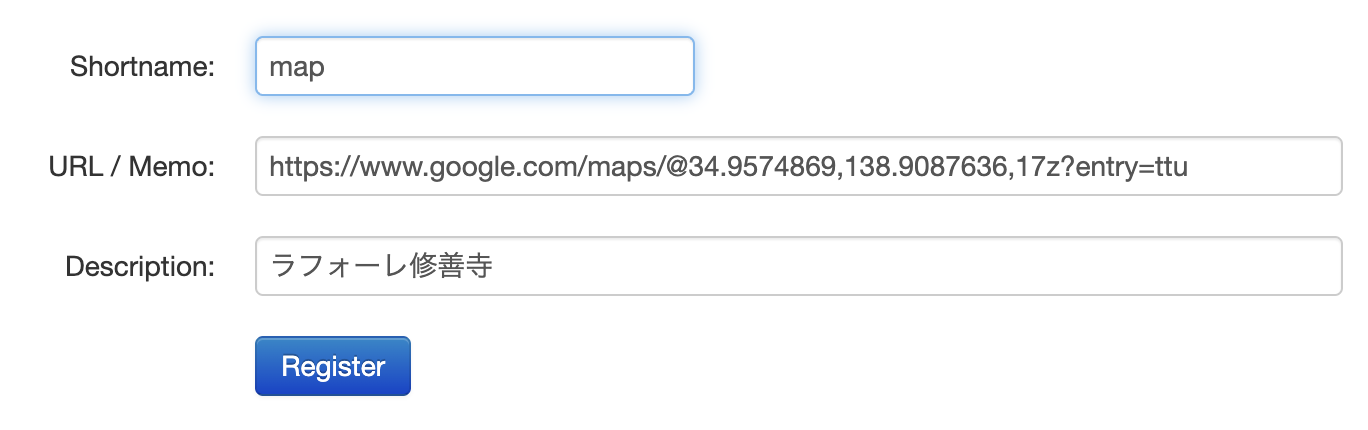
\includegraphics[width=10cm,bb=0 0 1368 430]{figures/bc5239609c72ac3054e0b4469bb4c037.png}
  \caption{GoQuickでラフォーレ修善寺を「map」と登録.}
  \label{shuzenji}
\end{figure}

\ref{mykw}で述べた
独自のキーワード検索に失敗した場合はショートカットが利用される。
ショートカットがGoQuickに定義されていない場合は
通常のWeb検索が行なわれる。

\subsection{答を直接取得}

たとえば、
ラフォーレ修善寺の電話番号を知るために検索エンジンを利用すると
以下のような手順を踏むのが普通である。

\vspace{2mm}

\begin{enumerate}
\item ラフォーレ修善寺のWebページを検索する
\item ラフォーレ修善寺のページに移動する
\item 「アクセス」のタブに移動する
\item 電話番号をみつけてコピーする
\end{enumerate}

\vspace{3mm}

住所の検索には住所録データベースを利用し、
電話番号は電話帳で管理する人も多いだろうが、
電話帳の場合は以下のようになるだろう

\vspace{2mm}

\begin{enumerate}
\item 電話番号を電話帳に記録したことを思い出す
\item 電話帳を開く
\item ラフォーレ修善寺を検索する
\item 電話番号をコピーする
\end{enumerate}

\vspace{3mm}
\noindent
いずれにしてもかなりの手間がかかってしまう。

一般的な検索エンジンやブックマークを利用するとき、
本当に欲しい情報に直接アクセスできないことが多い。

どこに記録したのか忘れてしまいがちだし、
住所録や電話帳を調べるインタフェースは独自のものとなってしまう。

電話番号や住所の文字列だけ知りたいときは、
\textbf{Oumugaeshi}というサービス\footnote{
  \textsf{http://oumugaeshi.com/}
}を利用すると良い。
ラフォーレ修善寺の電話番号が表示されるようなURLを
図\ref{tel}のように作成しておく。

\begin{figure}[h]
  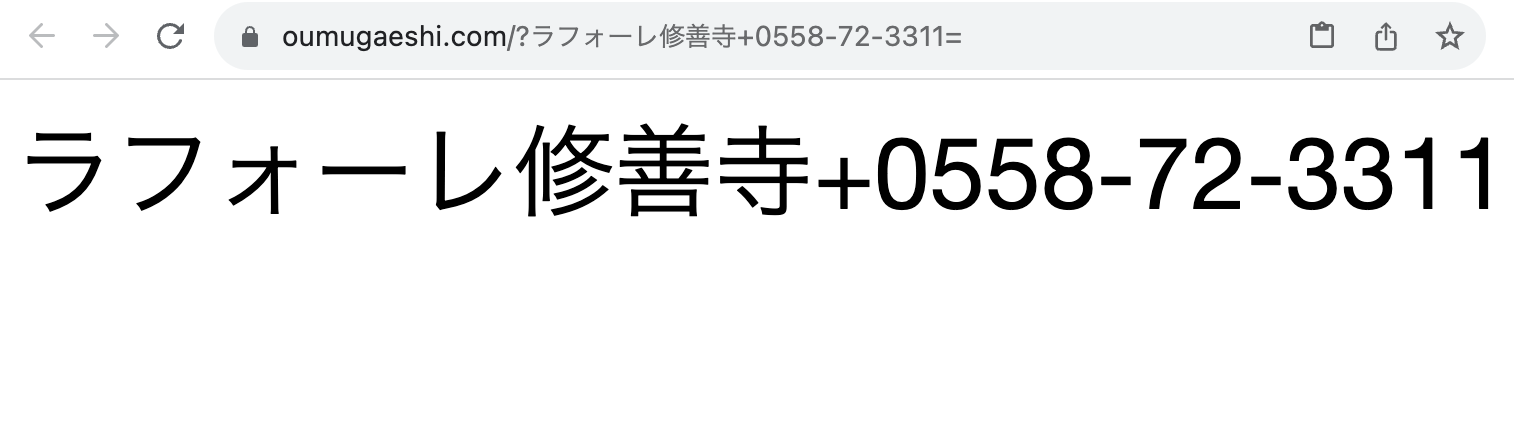
\includegraphics[width=10cm,bb=0 0 1514 434]{figures/41af781b930c1e4594ad53bdf429b4e9.png}
  \caption{ラフォーレの電話番号を示すURL.}
  \label{tel}
\end{figure}

このページに対して{\ds}で
「ラフォーレ修善寺の電話番号」のようなキーワードを登録しておけば、
図\ref{rafu}のように検索を行なって答を選択することにより、
図\ref{tel}のようなOumugaeshiのページを直接表示することができる。

\begin{figure}[h]
  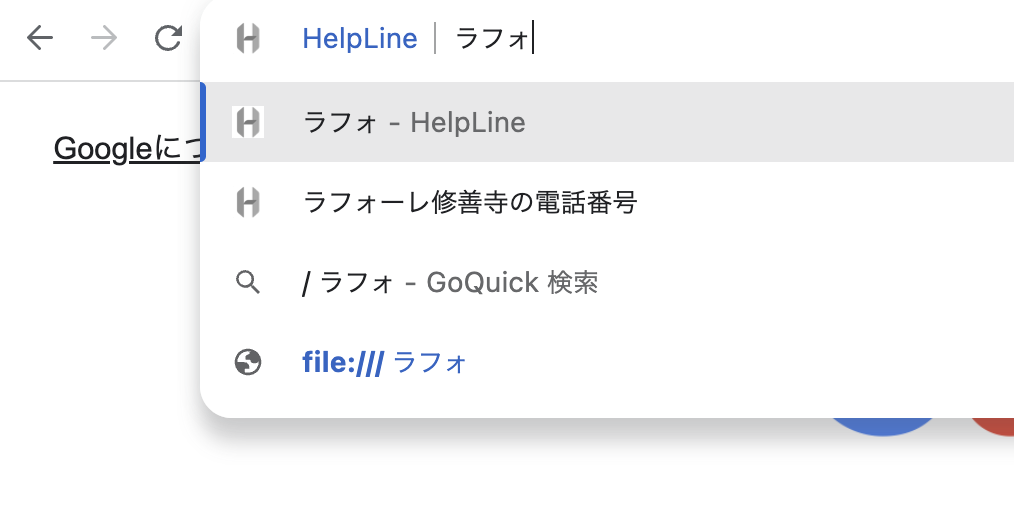
\includegraphics[width=10cm,bb=0 0 1014 514]{figures/ea7daea727f0669fedbb7ebb6567b23c.png}
  \caption{「ラフ」での検索結果.}
  \label{rafu}
\end{figure}

\section{実装}

{\ds}はChromeブラウザの拡張機能として実装されている。
データベースはブラウザのLocalStorage\footnote{
  \textsf{https:{\slash}{\slash}developer.mozilla.org{\slash}ja{\slash}docs{\slash}Web{\slash}API{\slash}Web\_Storage\_API}
}に格納され、JSON型式でインポート/エクスポートできる。

Karabiner-Elements\footnote{
\textsf{https:{\slash}{\slash}karabiner-elements.pqrs.org{\slash}}
}を利用し、
図\ref{3keys}の「H」のキーを押すと{\ds}が起動するようにしている。

\begin{figure}[h]
  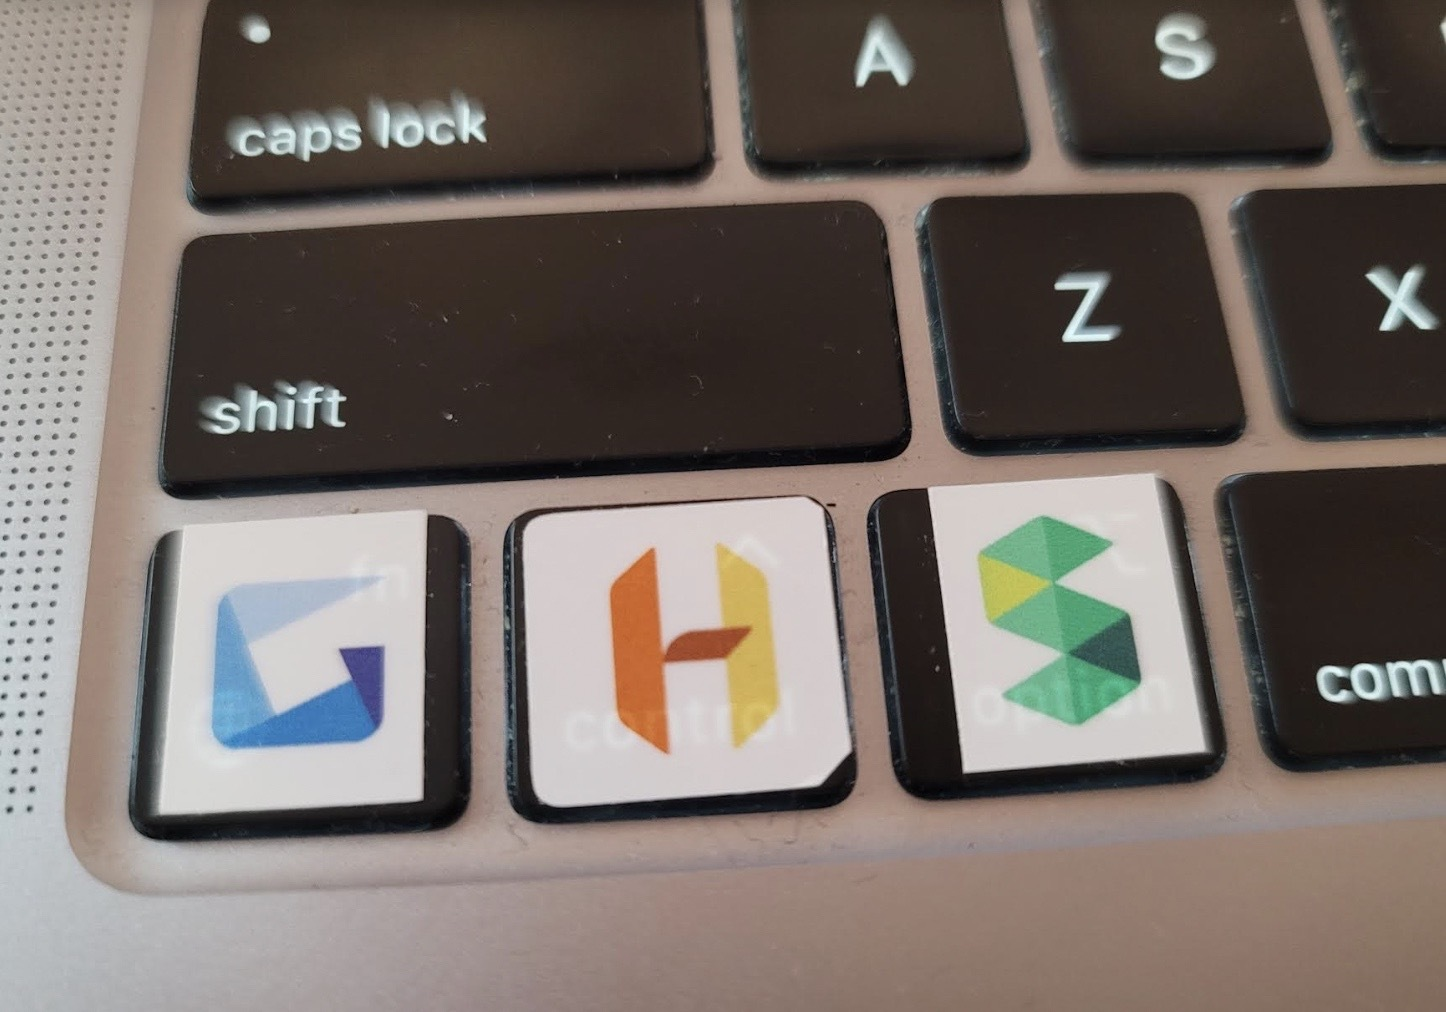
\includegraphics[width=10cm,bb=0 0 1446 1012]{figures/5a432cf5753e954ceb0069d0dbb5cde4.jpg}
  \caption{キーボードへの割り当て.}
  \label{3keys}
\end{figure}

% \begin{acknowledgment}
% 謝辞が必要であれば,ここに書く.
% \end{acknowledgment}

\section{評価と将来課題}

どのような検索対象であっても同じ検索システムが利用できるのは極めて便利である。
日常生活で検索を行なうとき、
「どこに置いたか」「どこで捜せば良いか」がわからなくなって苦労することは多いものだが、
あらゆる情報を{\ds}で検索できるようにしておけば
そのような精神的負担はなくなる。

ちょっとした情報を{\ds}で検索できるのは便利なので何でも記述しておきたくなるが、
不要になった情報は簡単に消せるようにしたい。

また、有用な情報を他人と共有するための仕組みが必要と考えている。


\begin{thebibliography}{9}
\bibitem{expandhelp} 増井俊之: 展開ヘルプ. インタラクション2012論文集, pp.89-96, March 2012.
\end{thebibliography}

\end{document}
